% ------------------------------------------------------------------------
% Template zur Erstellung von Seminararbeiten an der Professur für
% Digitalisierung, E-Business und Operations Management
% Erstellerin: Jella Pfeiffer
% Datum 08.10.2019
% Überarbeitet von Pascal Heßler am 19.08.2020
% ------------------------------------------------------------------------

% ------------------------------------------------------------------------
% Allgemeine Einstellungen
% ------------------------------------------------------------------------
\documentclass[12pt]{article}

\usepackage[paper=a4paper,left=30mm,right=30mm,top=40mm,bottom=40mm]{geometry}
\usepackage[utf8]{inputenc}       % Damit können Umlaute ganz normal geschrieben werden.
% \usepackage[english]{babel}       % Verwende deutsche, bzw. amerikanische Silbentrennung
\usepackage[ngerman]{babel}       % Deutsche Alternative
\usepackage{setspace}             % Zeilenabstand imlpementiert den Befehl 
% ------------------------------------------------------------------------
% Literatur
% ------------------------------------------------------------------------
% Achtung zur Einbindung der Literatur wird hier Biber verwendet und nich der Standard BibTex. In Sublime bracu man nichts verändern.
% 1. Sicherstellen, dass Biber installiert ist ->  in Tex Live vorinstalliert
% 2. Stellt eure Schreibumgebung um -> In TeXstudio: Optionen -> TeXstudio konfigurieren -> Erzeugen -> Standard Bibliographieprogramm
\usepackage[backend=biber,style=apa,natbib=false]{biblatex}
\DeclareLanguageMapping{american}{american-apa}         % Sprach Einstellung
\addbibresource{BibliographieAbschlussarbeit.bib}       % Legt die Datei fest in der die Literatur liegt (z. B.: Export aus Citavi)
\usepackage{breakcites}                                 % Falls Zitationen nicht ans Zeilenende passen
\usepackage{csquotes}                                   % Erweitert die Möglichkeiten beim zitieren
% ------------------------------------------------------------------------
% Mathematische Symbole
% ------------------------------------------------------------------------
\usepackage{amssymb}
\usepackage{amsmath}        % Formattierung von Tabellen und Matritzen
\usepackage{amsfonts}

% ------------------------------------------------------------------------
% Grafiken
% ------------------------------------------------------------------------
\usepackage{graphicx}       % Zum Einbinden von Grafiken
\usepackage{subfigure}      % Um Bilder innerhalb einer Figure anzuordnen (Bild a b c d...)

% ------------------------------------------------------------------------
% Tabellen
% Um einfache Tabellen zu erstellen kann https://www.tablesgenerator.com/ verwendet werden.
% ------------------------------------------------------------------------
\usepackage{tabularx}       % Ermöglicht weitere Tabellen Einstellungen
\usepackage{multirow}       % Ermöglicht Zellen zu verbinden
\usepackage{booktabs}       % Tabellen Midline Topline etc.
\usepackage{float}          % Tabelen Positionierung
\usepackage{longtable}      % Ermöglicht Tabellen über mehrere Seiten hinweg, so dass sie noch dasselbe Format besitzten ftp://ftp.fu-berlin.de/tex/CTAN/macros/latex/required/tools/longtable.pdf
% **********************************************************************************************************************
% Folgende Pakete sind rein optional und etwas komplexer in ihrer Umsetzung nur für etwas erfahrenere LaTeX User
% **********************************************************************************************************************
% \usepackage{siunitx}      % Ausrichten von Tabellen an dezimalstellen (Umsetzung etwas komplizierter)
% \usepackage{rccol}        % Ein Neues Format R (wird wahrscheinlich mit dem Folgenden R zu Problemen führen) und sorgt, dass nach , ausgerichtet wird und automatisches runden in Tabellen wird ermöglicht
% \usepackage{fltpoint}     % Gehört zu rccol
% \usepackage{dcolumn}      % Gehört zu rccol
%
% \newcolumntype{L}[1]{>{\raggedright\arraybackslash}p{#1}}       % Linksbündig mit Breitenangabe
% \newcolumntype{C}[1]{>{\centering\arraybackslash}p{#1}}         % Zentriert mit Breitenangabe
% \newcolumntype{R}[1]{>{\raggedleft\arraybackslash}p{#1}}        % Rechtsbündig mit Breitenangabe
% \newcolumntype{x}[1]{!{\centering\arraybackslash\vrule width #1}}
% ------------------------------------------------------------------------
% Lua Wordcount
% ------------------------------------------------------------------------
\usepackage{luacode}
% loads lua script
\directlua{dofile(kpse.find_file"word_count.lua")}
% defining latex commands to use lua functions easier 
\def\setwordthreshold#1{
  \directlua{packagedata.word_count.set_threshold(\number#1)}%
}

\def\startwordcount{
  \directlua{
    luatexbase.add_to_callback(
    "pre_linebreak_filter",
    packagedata.word_count.callback,
    "word_count"
    )
  }
}

\def\stopwordcount{
  \endgraf %% force paragraph
  \directlua{
    luatexbase.remove_from_callback(
    "pre_linebreak_filter",
    "word_count"
    )
  }
}

% Creates Logfile
\def\dumpwordcount{%
  \directlua{packagedata.word_count.dump_total_word_count()}
}
% This returns the normalized sides at the current position
\def\dumprelativwordcount{%
  \directlua{packagedata.word_count.dump_relativ_word_count()}%
}

% This returns the word count at the current position.
\def\currentwordcount{%
  \directlua{packagedata.word_count.current_word_count()}
}

% Text result
\def\prettyresult{\directlua{packagedata.word_count.pretty_result()}}

% ------------------------------------------------------------------------
% Sonstige
% ------------------------------------------------------------------------
\usepackage{scrhack}        % Löst unnötige Warnungen!
\usepackage{color}          % Ermöglicht Text einzufärben \pagecolor{FARBE}  \color{FARBE} \textcolor{FARBE}{TEXT} \colorbox{FARBE}{TEXT}
\usepackage{hyperref}       % Ermöglicht URLS schreibweise ist z.B. \url{http://www.uni-giessen.de}

\usepackage{eurosym}        % Für Euro Symbol \euro{} oder \eruo (Unterschieden sich bezüglich Leerzeichen danach)

\usepackage{framed}         % Einrahmen von Texten mit der shaded-Umgebung.

\usepackage{pdflscape}      % Querformat möglich über \begin{landscape} \end{landscape}
% ------------------------------------------------------------------------
% Fein Justierungen
% ------------------------------------------------------------------------
\DeclareMathOperator*{\argmax}{arg\,max}

\newenvironment{packed_enum}{
\begin{enumerate}
  \setlength{\itemsep}{1pt}
  \setlength{\parskip}{0pt}
  \setlength{\parsep}{0pt}
}{\end{enumerate}}

\hypersetup{hidelinks}                 % Versteckt die Links im PDF (optisch)
% ----- ende der präambel ----------------------------------
% Start des Dokuments
% ----------------------------------------------------------
\begin{document} 
% Theoretisch kann man auch alles in einem Dokument haben. Das ist jedoch unübersichtlich. Daher werden hier die einzelnen Kapitel eingebunden.
\pagenumbering{Alph}                  % Löst unnötigen Warnungen
% Die Titelseite der Arbeit

\begin{titlepage}
\begin{center} % zentrieren

  % Logo der Uni Giessen bitte suchen und einfuegen
  \begin{figure}[ht]
    \centering
    
\includegraphics{graphics/logo.png}
  \end{figure}

  % Vertikaler Zwischenraum
  \bigskip
  \vfill
  % Titel der Arbeit und Typ der Arbeit, umrandet
    \begin{framed}
    \begin{center}
      \textsc{{\Large Titel\\
      Untertitel\\}}
                                % Letztes \\ ist wichtig, beginnt eine neue Zeile f{\"u}r die Art der Arbeit

      \bigskip

                                % Art der Arbeit, ggf. auszutauschen gegen Seminar- oder Bachelorarbeit
      \textbf{Seminararbeit}
    \end{center}
    \end{framed}
    \vfill
    \vfill


  % Daten des Erstellers, Einreichungsdatum
  % in einer Tabelle ausgerichtet
  \begin{tabular*}{0.62\textwidth}{r@{\extracolsep{\fill}}l}
    eingereicht im: & Oktober 2019\\\\
    von: & XXX\\
    & geboren am XX. Oktober 2010\\
    \\
    Matrikelnummer: & XXX\\
    Studiengang: & XXX\\
    Private Adresse: & XXX\\
    Telefonnummer: & XXX\\
    E-Mail-Adresse: & XXX
  \end{tabular*}
  \vfill
  \vfill


  \rule{\textwidth}{.4pt}\\ % vertikale Linie
  Justus-Liebig-Universität Gießen\\
  Professur f\"ur Digitalisierung, E-Business und Operations Management\\
  35394  Gie\ss{}en\\
  \small \url{https://www.uni-giessen.de/fbz/fb02/fb/professuren/bwl/e-business-operations-management}
\end{center}

\end{titlepage} % Ende des Titelblatts

%%% Local Variables:
%%% mode: latex
%%% TeX-master: "~/Documents/DA-Vorlage/beispiel/da-beispiel"
%%% End:
              % Titelseite einbinden
\pagenumbering{arabic}                % Löst unnötigen Warnungen
%!TEX root = ../master.tex
\section*{Abstract}
[Hier ein Beispiel für ein Abstract. Ihr Abstract sollte 150-250 Wörter haben] We investigate how each of the two steps that are typically supported by purchasing platforms ― filtering and joint evaluation ― affects the success of a prosocial microlending platform. Users of such platforms lend money interest-free to people in need, such as small-scale entrepreneurs from developing countries. We hypothesize that while attribute-based filtering can reduce the decision effort and provide guidance, which is often perceived as helpful in purchasing decisions, it may be perceived as inappropriate and restrictive in the prosocial microlending domain, thereby reducing users’ choice satisfaction. Building on evaluability theory, we further hypothesize that joint evaluation is a double-edged sword: Jointly evaluating more than one alternative increases choice satisfaction by facilitating evaluability, as alternatives can serve as reference points, and because not being able to compare alternatives could feel restrictive. However, jointly evaluating alternatives also highlights conflicts and tradeoffs between alternatives and thereby decreases users’ willingness-to-contribute to the alternative they finally choose. We test our hypotheses in an incentivized lab experiment, using real prosocial lending decisions. Our findings suggest that offering attribute-based filters does not increase a platform’s success, and confirm that joint evaluation is a double-edged sword. Platforms have to trade off decreased choice satisfaction with increased willingness-to-contribute.

\newpage

\onehalfspacing
% ------------------------------------------------------------------------
% Hauptarbeit (hier werden alle Kapitel eingebunden)
% ------------------------------------------------------------------------
\setwordthreshold{2}                   % min chars in a row to count as word
\startwordcount                        % start counting words

%!TEX root = ../master.tex
\section{Introduction} \label{sec:introduction}

Wissenschaftliche Arbeiten weisen standardisierte Strukturen auf, von denen man im Aus- nahmefall abweichen kann. Eine Standardstruktur für empirische Arbeiten ist die folgende:
\begin{itemize}
  \item Abstract
  \item Introduction [Einleitung]
  \item Related Work [Grundlagen und Verwandte Arbeiten]
  \item Method/Experimental Design/Implementation
  \item Results
  \item Discussion
  \item Conclusions
  \begin{itemize}
    \item Summary (ist optional!)
    \item Limitations and Future Research [Limitationen und Ausblick]
     \item Contribution [Fazit/Schlussfolgerung]
   \end{itemize}
   \item References [Literaturverzeichnis]
   \item Appendix [Anhang]
\end{itemize}


Literaturbasierte Arbeiten verfolgen weniger eine Standardstruktur. Orientieren können Sie sich heran:
\begin{itemize}
  \item	Abstract
  \item Introduction [Einleitung]
  \item Related Work [Grundlagen und Verwandte Arbeiten]: Es kann sein, dass Sie dieses Kapitel besser über mehrere Kapitel mit unterschiedlichen Schwerpunkten verteilen und diese dann auch spezifisch in der Kapitelüberschrift entsprechend des Inhalts benennen (und nicht einfach related work).
  \item Method/Experimental Design/Implementation: Dieses Kapitel sollten Sie weglassen, falls Sie nicht viel zu Ihrer Methodik sagen können. Aber selbst wenn Sie nur eine literaturbasierte Arbeit und keine empirische Schreiben, können Sie hier sehr strukturiert vorgehen und dann hier Ihre Literaturarbeit beschreiben, z.B. nach welchen Keywords haben Sie gesucht und wo, welche gefundene Quellen haben Sie ein/ausgeschlossen, etc..
  \item Results: Dieses Kapitel heißt oft anders in rein literaturbasierten Arbeiten und hat dann einen für die Arbeit spezifischen Titel, wie z.B. Risiko-Nutzen-Analyse der Einführung von Industrie 4.0. Hier ist der Teil, der größten Eigenleistung, in der Sie selbst interpretieren, Frameworks formulieren, Modelle formulieren oder ähnliches
       \item Conclusions
  \begin{itemize}
    \item Summary (ist optional!)
    \item Limitations and Future Research [Limitationen und Ausblick]
     \item Contribution [Fazit/Schlussfolgerung]
   \end{itemize}
  \item References [Literaturverzeichnis]
  \item Appendix [Anhang]
\end{itemize}

Die typische Struktur der Einleitung ist:
\begin{enumerate}
  \item Problemstellung und Motivation
  \item Stand der Forschung, darauf aufbauend Forschungslücke und Forschungsfrage(n) herausarbeiten
  \item Ziel der Arbeit und eigener methodischer Ansatz zur Beantwortung der Forschungsfrage(n): Absatz beginnt meist mit: The goal of this thesis/work/manuscript is
  \item Ergebnisse der Arbeit [optional]
  \item Erwarteter wissenschaftlicher (und praktischer) Beitrag [=Contribution]
  \item Manchmal folgt noch eine Gliederung [ausformuliert]
\end{enumerate}

\section{Figures and Tables} \label{sec:figuresTables}

Hier finden Sie nun Beispiele für das einfügen von Grafiken und Tabellen. Für Tabellen können Sie auch Umgebungen wie tabularx und longtable verwenden.

We performed experiments for three different product categories ranging from commodity products (energy-saving lamps) over hotel rooms to capital goods (washing machines). A lower average price of the products represents a lower perceived risk. We used energy-saving lamps as rather low priced products (avg.\ price: 7.57\euro), hotel rooms as medium priced products (avg.\ price: 249.50\euro) and washing machines as rather high priced products (avg.\ price: 524.33\euro). For each category, we collected data for 40 products. Each product is described by five attributes. Specifically, we extracted frequently used attributes from Amazon product descriptions (energy-saving lamps, washing machines) or descriptions in the hotel booking platform HRS. Table \ref{tab:productsExp1} summarizes products and product attributes\footnote{For washing machines and energy-saving lamps, consumer ratings are from Amazon; for hotel rooms, consumer ratings are from hrs.com. The attribute level order for washing machine brands is based on the brands' average sales rank on Amazon.}.

 \begin{table}[!h]
	\caption{Products and their Attributes}\label{tab:productsExp1}
	\begin{center}\small
		\begin{tabularx}{15cm}{llll}
			\hline
			Product & Attribute & Unit & Attribute Level Order\\
			\hline
			Energy-saving & Price & Euro & Increasing \\
      Lamp& Energy Efficiency Grade & -- & A+ $\succ$ A $\succ$ B  \\
      (n=40)& Deviation from Day Light & -- & None $\succ$ Low $\succ$ Large \\
      & Durability & Hours working time & Decreasing \\
      & Customer Rating & 1-5 Stars & Decreasing \\
			\hline
			Hotel Room & Price per Night & Euro & Increasing \\
      (n=40)& Category & Stars & Decreasing \\
      & Distance from City Center & Kilometers & Increasing \\
      & WLAN availability & -- & Available $ \succ$ Not available \\
      & Customer Rating & 1-5 Stars & Decreasing \\
			\hline
			Washing & Price & Euro & Increasing \\
      Machine& Brand & -- & Siemens $\succ$ Bosch $\succ$ AEG \\
      (n=40)& & & $\succ$ Bauknecht $\succ$ Gorenje \\
      & & & $\succ$ Blomberg $\succ$ LG \\
      & Energy Consumption & kWh per year & Increasing \\
      & Water Consumption & Liters per year & Increasing \\
      & Customer Rating & 1-5 Stars & Decreasing \\
			\hline			
      \multicolumn{3}{l}{$\succ$\emph{: is preferred over}}
		\end{tabularx}
	\end{center}
\end{table}

\begin{figure}[t]
  	\caption{Example Product Domination Graph}\label{fig:productGraph}
  	\begin{center}
 		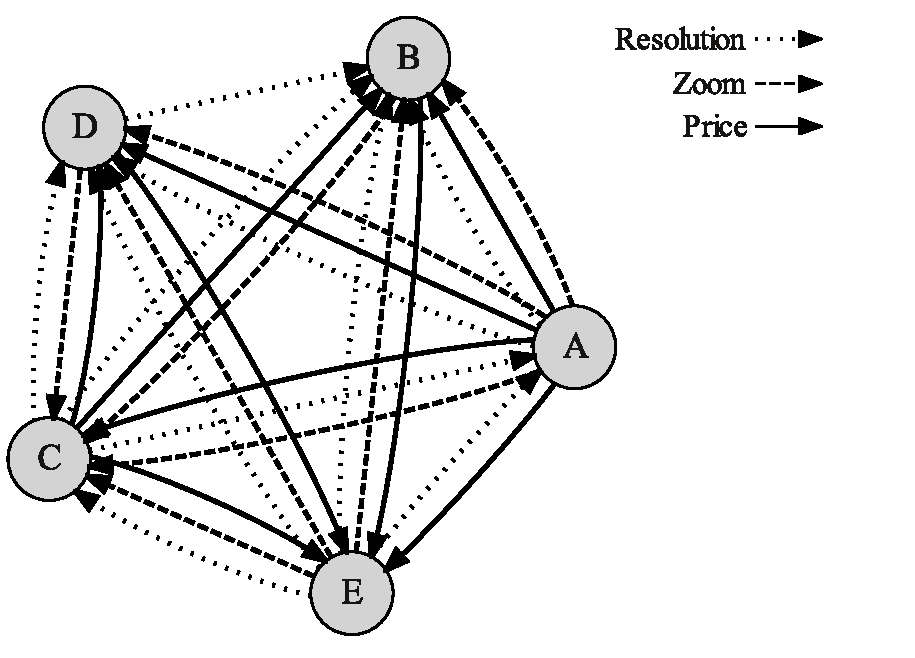
\includegraphics[width=10cm]{graphics/ProductDominationGraph}
 	\end{center}
\end{figure}

Let us give an example. We assume a choice scenario with five different cameras (see Table \ref{tab:cameras}). Product attributes are photo resolution $ph$, zoom factor $zf$, and price $pr$. All consumers have the same preference for the attribute level order: they prefer lower to higher prices, and higher photo resolutions and zoom factors to lower ones. Table \ref{tab:cameras} lists the five exemplary cameras with their corresponding attribute levels as well as single-attribute values $v_{i}$ for each attribute $a_i\in\{ph, zf, pr\}$.
Camera $E$ has the best price, but the worst photo resolution. In the product domination graph, $E$ has hence no outgoing edges with respect to price, but four outgoing edges with respect to photo resolution. Figure \ref{fig:productGraph} shows the resulting product domination graph.

Eine Tabelle finden Sie in Tabelle \ref{tab:cameras}.
\begin{table}%[!h]
	\caption{Example attribute levels and corresponding single-attribute values $v_i$}\label{tab:cameras}
	\begin{center}\small
		\begin{tabular}{lrrr}  		
			\hline
			Camera & Photo Resolution & Zoom Factor & Price\\
			\hline
			A & $v_{ph}(12 MP) = 0.60$ & $v_{zf}(10x) = 0.00$ & $v_{pr}(610 EUR) = 0.00$\\
			B & $v_{ph}(14 MP) = 1.00$ & $v_{zf}(15x) = 0.63$ & $v_{pr}(470 EUR) = 0.40$\\
			C & $v_{ph}(10 MP) = 0.20$ & $v_{zf}(18x) = 1.00$ & $v_{pr}(540 EUR) = 0.20$\\
			D & $v_{ph}(13 MP) = 0.80$ & $v_{zf}(15x) = 0.63$ & $v_{pr}(470 EUR) = 0.40$\\
			E & $v_{ph}(9 MP) = 0.00$ & $v_{zf}(10x) = 0.00$ & $v_{pr}(260 EUR) = 1.00$\\
			\hline
		\end{tabular}
	\end{center}
\end{table} 	


%!TEX root = ../master.tex
\section{Combinatorial Auctions}
\label{chap:combinatorialAuctions}

Die ist der Ausschnitt eines Beispielkapitels.

\emph{Combinatorial auctions} (CAs) are a part of electronic
market design. Research in electronic market design joins two
disciplines: economics and computer science. Economical research
focuses on game theoretical aspects by analyzing strategic
behavior of self-interested agents. From the viewpoint of computer
science, computational problems are addressed, such as finding the
optimal allocation in auctions. As this work concentrates on
computational aspects, we assume that the reader has a stronger
background in computer science than in economics. Thus, in this
chapter we will point out the main ideas of the economical
perspective to provide some basic knowledge in this area.

\section{Mechanism Design}
\subsection{Definition}
Mechanism design was introduced by \textcite{Hu60}. It
aims at implementing system-wide solutions to problems in
non-cooperative environments with multiple self-interested agents.
Such problems can be political elections, public projects in which
the participants themselves have to invest money, or allocation
problems. Given that agents hold only private information about
their preferences, a structure has to be chosen in which in
equilibrium each agent behaves according to the designer's or principal's
intentions. The designer can either act on behalf of the society, for
example when collecting taxes for a public project, or she can
pursue self-interests when, for instance, being an auctioneer.

Since the agents' information is private, the principal faces the
problem that the agents might lie about their real valuations in
order to influence the outcome according to their preferences. In
most cases, whenever such manipulations occur, they damage the
resulting system-wide welfare \parencite{NiRo00}. Thus, simply asking
the participants to reveal their preferences is unfavorable.
Therefore, the principal has to define other rules which lead to
the desired outcome. The most common solution to this problem is
to introduce monetary transfers providing incentives for the
agents to behave truthfully.

In mechanism design two economic areas are joined: \emph{game
theory} and \emph{social choice theory}. In game theory the
agents' strategies are analyzed, and in social choice theory an
outcome is selected according to a set of agents' preferences. The
outcome in social choice theory is determined by a social choice
function, which is to be implemented by a mechanism. Formally we
have a set of possible outcomes $O$ and agents $i \in I$, $|I|=n$.
Each agent $i$ has a type $\theta_i \in \Theta_i$ reflecting the
possible preference sequences the agent can have. The type captures
all of the agent's private information relevant to her decision.
The agent's utility $u_i(o,\theta_i)$ over each outcome depends on
her type; while $u_i(o_1,\theta_i)>u_i(o_2,\theta_i)$ means that
the outcome $o_1$ is preferred over the outcome $o_2$. The social
choice function maps from the space of all types $\Theta$ to the
space of all outcomes $O$,
\begin{eqnarray}
% \nonumber to remove numbering (before each equation)
  f:\Theta_1 \times\Theta_2\times...\times\Theta_n\rightarrow O.
\end{eqnarray}
Examples for such social choice functions are allocation problems or political voting
protocols in which a candidate or a party is chosen. The most common objective of a social choice function is
the maximization of the social welfare, the so called
\emph{allocative-efficiency} \parencite{Pa01}. It maximizes the sum of
all utilities over all agents:
\begin{eqnarray}
\label{Efficient}
% \nonumber to remove numbering (before each equation)
  f(\theta)=\argmax_{o \in O} \sum_{i \in I} u_i(o,\theta_i).
\end{eqnarray}
Another objective is \emph{individual rationality}; the agent's
payoff is never less when participating in the mechanism than her
payoff without participating. Additionally there is \emph{Pareto
optimality}. An outcome is Pareto optimal whenever none of the
agents could perform better without causing another agent to
perform worse than in the current situation.

So far, we have learned what a social choice function is, and what
typical objectives for the choices of outcomes are. Now, a
mechanism has to be found which implements a given social choice
function with one or several of these objectives. For this
purpose, the agents' possible strategies have to be specified
together with an outcome function based on these strategies. The
mechanism should guarantee an implementation despite the
self-interest of the agents \parencite{Pa01}. Mathematically, a
mechanism $M$ is defined on the strategy spaces $S_i$ of the
agents:
\begin{equation}\label{MechanismDefinition}
  M=((S_1,...S_n),g(\cdot))\\
  g:S_1\times...\times S_n\rightarrow O,
\end{equation}
where $g$ is an outcome function and $S_i$ denotes all strategies
or actions an agent $i$ is allowed to take. A mechanism implements
a social choice function if there is an equilibrium strategy
profile $s^\ast(\cdot)=(s^\ast_1(\cdot),...,s^\ast_n(\cdot))$ of
the game induced by $M$ so that
\begin{equation}\label{MechanismImplements}
    g(s^\ast_1(\theta_1),...,s^\ast_n(\theta_n))=f(\theta_1,...,\theta_n),
      \quad \forall
      (\theta_1,...,\theta_n)\in(\Theta_1,...,\Theta_n),
\end{equation}
where $s^\ast_i(\theta_i)$ is the strategy agent $i$ with type
$\theta_i$ plays in the equilibrium. Please note that the
equilibrium concept is not specified in this definition. It could,
for example, be a Nash equilibrium. In this case, given the other
players $j,$ $j \neq i$, conform to the equilibrium strategies
$s^\ast_j(\theta_j)$, no other player $i$ has an incentive to
unilaterally deviate from her equilibrium strategy. Other examples
are the dominant strategy or the Bayes-Nash strategy equilibrium.
The dominant strategy equilibrium facilitates it for the agents
since the optimal strategy for an agent is independent of any
strategies the other agents could play. Thus, the agents do not
need to speculate about the way the others might behave. Informally,
we could say that the concept of dominant strategies "removes game
theory from the problem" \textcite[p.~5]{Pa01}. The Bayes-Nash
equilibrium is similar to Nash equilibriums, but assumes that
agents have incomplete information about the opponents' types.
Therefore, agents use probability functions to speculate about the
other agents' preferences \parencite{OsRu94}.

\subsection{Revelation Principle and Gibbard-Satterthwaite Theorem}
In equation \ref{MechanismDefinition}, we see that a mechanism
defines the available strategies and the function for selecting an
outcome. It is necessary that these strategies are kept simple so
that they can be applied by the agents. The easiest strategies
occur when choosing a \emph{direct mechanism} asking the agents to
report their types directly to the principal, $S_i=\Theta_i$.
Direct mechanisms lead to a centralization of the problem as
agents report their types to a center that determines the outcome
and reports it back to the agents. On the contrary, when applying
\emph{indirect mechanisms} agents have to think about how to
transform their type into a strategy and the latter is reported to
the mechanism. In other words,
\begin{quote} "the computations that go on within the mind of any
bidder in the non-direct mechanism are shifted to become part of
the mechanism in the direct mechanism". \textcite[p.~712]{McMc87}
\end{quote}
When applying these direct mechanisms agents may still lie about
their true types. Mechanisms which, in contrast, succeed in
establishing an equilibrium in which all agents tell the truth,
are called \emph{incentive-compatible}. In this case, it is in the
interest of all agents to report their true types,
$s^\ast_i(\theta_i) = \theta_i,~\forall \theta_i \in \Theta_i$.
Further, if telling the truth is a dominant strategy, the
mechanism is called \emph{strategy-proof}. As will be shown later
on, this can be achieved by the \emph{Vickrey-Clarke-Grooves}
(VCG) mechanism.

We learned that the equilibrium strategy profile $s^\ast(\cdot)$
does not determine the concept of equilibrium. Some equilibrium
concept must be chosen and implemented together with the mechanism. In the
worst case, in order to find out if a certain social choice
function can be implemented by a certain mechanism with, for
instance, dominant strategies, one would have to consider all
possible mechanisms. However, research on mechanism design led to
the \emph{revelation principle} as a solution to this. It states
that for any mechanism, there is a direct, incentive-compatible
mechanism with the same outcome \parencite{McMc87}. An intuitive
explanation for this principle consists in: the transformation
from types into strategies, which occurs in the agents' minds in
indirect mechanisms, and which is used as a filter in the direct mechanism.
That is, the direct mechanism first filters all reports of the
agents and simulates the indirect mechanism with the filtered
input. This principle is valid for the optimal mechanism as well.
Thus, the search for a mechanism can focus on direct
mechanisms. Therefore, if no direct mechanism can implement a
given social choice function, then no indirect mechanism will do
so.

In contrast to the positive result of the revelation principle,
there also exists a negative result, the
\emph{Gibbard-Satterthwaite} theorem. According to it, it is
impossible to find a mechanism with certain positive
characteristics. To understand the theorem, first note that a
social choice function is \emph{truthfully implementable} if and
only if the dominant strategy is to reveal the truth. Furthermore,
a social choice function $f$ is \emph{onto} if for each $o \in O$
at least one element in $\Theta$ exists so that $f$ maps to $o$.
Finally, a social choice function $f$ is \emph{dictatorial}
whenever there is a dictator $j$ among the agents so that for all
outcomes, $o_j$ is strictly preferred to another outcome $o_k$
whenever the dictator $j$ strictly prefers $o_j$ to $o_k$.
Obviously, this is an unwanted characteristic. It turns the
Gibbard-Satterthwaite theorem impractical for real-life mechanisms
since they allow manipulation.

\textbf{Gibbard-Satterthwaite Theorem:} \emph{Given $O$ is finite,
$|O|\geq 3$, and the social choice function $f$ is onto, then $f$
is truthfully implementable in dominant strategies if and only if
f is dictatorial}.

According to the theorem it is impossible to elicit the truth if
dominant strategies exist. However, despite this result, the
theorem can be circumvented by placing restrictions on the agents'
preferences, the way it is done in the VCG mechanism.

\subsection{Vickrey-Clarke-Grooves Mechanism}
The VCG mechanism combines the following important virtues by
introducing a special payment scheme. First, it implements social
choice functions in dominant strategies. Thus, agents do not have
to speculate which strategies the other agents might play, and
they do not need to waste resources on learning about their
competitors' strategies. Second, the mechanism does not have to
make any assumptions about the information agents have on each
other. And, third, the VCG mechanism is allocative-efficient (see
equation \ref{Efficient}), strategy-proof and non-dictatorial.

AND SO ON... 
%!TEX root = ../master.tex
\section{Conclusions}\label{chap:conclusions}

Auf Deutsch: Fazit. Je nach länge des Fazits, müssen sie dieses nicht weiterunterteilen.

\section{Summary}

Auf Deutsch: Zusammenfassung 

Die Zusammenfassung der Arbeit ist optional. Sollten Sie die Arbeit noch einmal zusammenfassen wollen, so halten Sie dies bitte eher kurz und wiederholen Sie sich nicht zu sehr.

\section{Limitations and Future Research}

Auf Deutsch: Limitationen und Ausblick

Es ist sinnvoll, jede Limitation an eine Idee zu knüpfen, wie diese in zukünftigen Arbeit zu adressieren waere.

\section{Contribution}

Auf Deutsch: Beiträge

Was sind die Beitraege Ihrer Arbeit sowohl für die Wissenschaft (und Theorie) als auch für die Praxis? Hier sollten Sie versuchen über den Tellerrand hinauszuschauen und einen eher weiten Blick einnehmen.






\stopwordcount                         % stopwordcount
\dumpwordcount                         % Cretaes log file
\prittyresult                          % Gibt im Fließtext Anzahl Wörter /Seiten aus --> Auskommentieren für die Abgabe!
% ------------------------------------------------------------------------
% Hauptarbeit ENDE
% ------------------------------------------------------------------------

% ------------------------------------------------------------------------
% Erstellen des Literaturverzeichnisses
% ------------------------------------------------------------------------
\printbibliography[heading=bibintoc]  
%!TEX root = ../master.tex
\section{Appendix}\label{Appendix}

\begin{table}[h]
\centering
\caption{Size of the search space for BASIC strategies ($n=4$).}
\label{tab:sizeSearchSpace}
 \begin{tabular}{r|r|r}
      m&s&search space size\\
      \hline
      4&1&64\\
      &2&4096\\
      &3&262,144\\
      &4&16,777,216\\
      &5&1,073,741,824\\
      7&1&262144\\
      &2&16777216\\
      &3&68,719,476,736\\
      &4&2.81E+14\\
      &5&1.15E+18\\
\end{tabular}
\end{table}



\section*{Selbstständigkeitserklärung}
\thispagestyle{empty}
Hiermit versichere ich, die vorgelegte Seminararbeit selbstständig und ohne unerlaubte fremde Hilfe und nur mit den Hilfen angefertigt zu haben, die ich in der Seminararbeit angegeben habe. Alle Textstellen, die wörtlich oder sinngemäß aus veröffentlichten Schriften entnommen sind, und alle Angaben die auf mündlichen Auskünften beruhen, sind als solche kenntlich gemacht. Bei den von mir durchgeführten und in der Seminararbeit erwähnten Untersuchungen habe ich die Grundsätze guter wissenschaftlicher Praxis, wie sie in der \glqq Satzung der Justus-Liebig-Universität zur Sicherung guter wissenschaftlicher Praxisext\grqq{} niedergelegt sind, eingehalten. Gemäß \S 25 Abs. 6 der Allgemeinen Bestimmungen für modularisierte Studiengänge dulde ich eine Überprüfung der Thesis mittels Anti-Plagiatssoftware.
\bigskip

\raggedright{Gießen, den XX.XX.XX} \bigskip \bigskip \bigskip

Ihr NAME


\end{document}
% ----------------------------------------------------------
% Ende
% ----------------------------------------------------------
